\chapter{Исследовательский раздел}
\label{cha:research}

В данном разделе описаны эксперименты, проводимые с разработанным программным обеспечением. Эксперименты проводятся с целью определения скоростных характеристик разработанного программного обеспечения и метода в целом, производится оценка точности обнаружения ситуаций гонок в программах в зависимости от их структуры.

\section{Условия проведения экспериментов}

Проведение экспериментов производилось в следующих условиях:
\begin{enumerate}
    \item аппаратное обеспечение:
        \begin{enumerate}
            \item AMD Turion(tm) X2 Ultra Dual-Core Mobile ZM-82 2,2GHz;
            \item 3096 Мб ОЗУ;
        \end{enumerate}
    \item программное обеспечение:
        \begin{enumerate}
            \item ОС Fedora GNU/Linux 20.0 3.11.10-301.fc20.i686;
            \item GCC 4.8.2;
            \item Python 2.7.5;
            \item gcc-python-plugin 0.12.
        \end{enumerate}
\end{enumerate}

\section{Исследование скоростных характеристик}

Для проведения экспериментов по определению скоростных характеристик за основу была взята задача <<читатели-писатели>>. В ней предполагается, что есть некоторый общий для всех потоков ресурс. Часть потоков получает к нему доступ только для чтения, а часть - для записи. При этом чтение может осуществляться одновременно из нескольких потоков. Код анализируемой программы представлен в листинге ~\ref{lst:readers-writers}.

\lstinputlisting[language=C,caption=Код решения задачи "читатели-писатели" (\Code{readers-writers.c}),label=lst:readers-writers]{inc/src/readers-writers.c}

В процессе проведения экспериментов проводилось изменение числа потоков, создаваемых в функции \textbf{main}, и ограничения, накладываемого на максимальное количество вхождений базового блока в анализируемый путь. Графики зависимостей количества анализируемых путей и количества анализируемых инструкций от изменения максимального количества вхождений базового блока в путь представлены на рис.~\ref{fig:graphic1} и на рис.~\ref{fig:graphic2} соответственно. Зависимости времени анализа от количества анализируемых путей, количества анализируемых инструкций и количества потоков представлены на рис.~\ref{fig:graphic3}, рис.~\ref{fig:graphic4} и рис.~\ref{fig:graphic5} соответственно. Видно, что с ростом ограничения, накладываемого на максимальное количество вхождений базового блока в путь, происходит экспоненциальный рост количества анализируемых путей и инструкций. Время анализа от количества анализируемых путей и инструкций зависит линейно. Повышение точности анализа с ростом значения ограничения, накладываемого на максимальное количество вхождений базового блокак в путь, не была выявлена, следовательно, разумно  в дальнейшем использовать при анализе значения данного ограничения, равным 1. Кроме того было выявлено, что количество созданных потоков слабо влияет на время анализа. Это объясняется тем, что анализ каждой функции программы выполняется только один раз, в местах, где производится её вызов, применяются результаты анализа, полученные ранее.

\begin{figure}
  \centering
  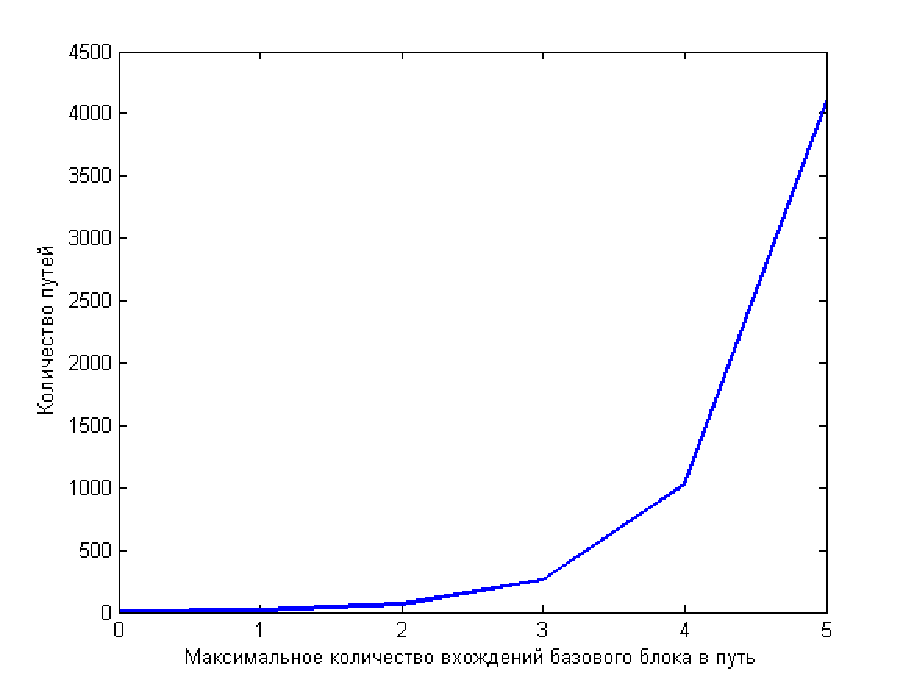
\includegraphics[width=0.9\textwidth]{inc/png/graphic1}
  \caption{Зависимость количества анализируемых путей от максимального количества вхождений базового блока путь}
  \label{fig:graphic1}
\end{figure}

\begin{figure}
  \centering
  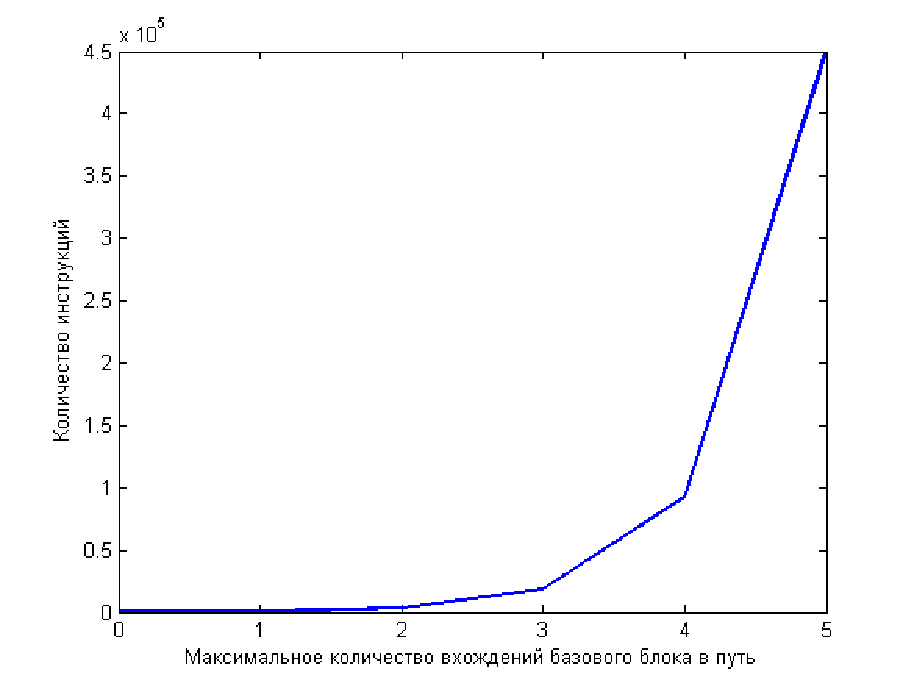
\includegraphics[width=0.9\textwidth]{inc/png/graphic2}
  \caption{Зависимость количества анализируемых инструкций от максимального количества вхождений базового блока путь}
  \label{fig:graphic2}
\end{figure}

\begin{figure}
  \centering
  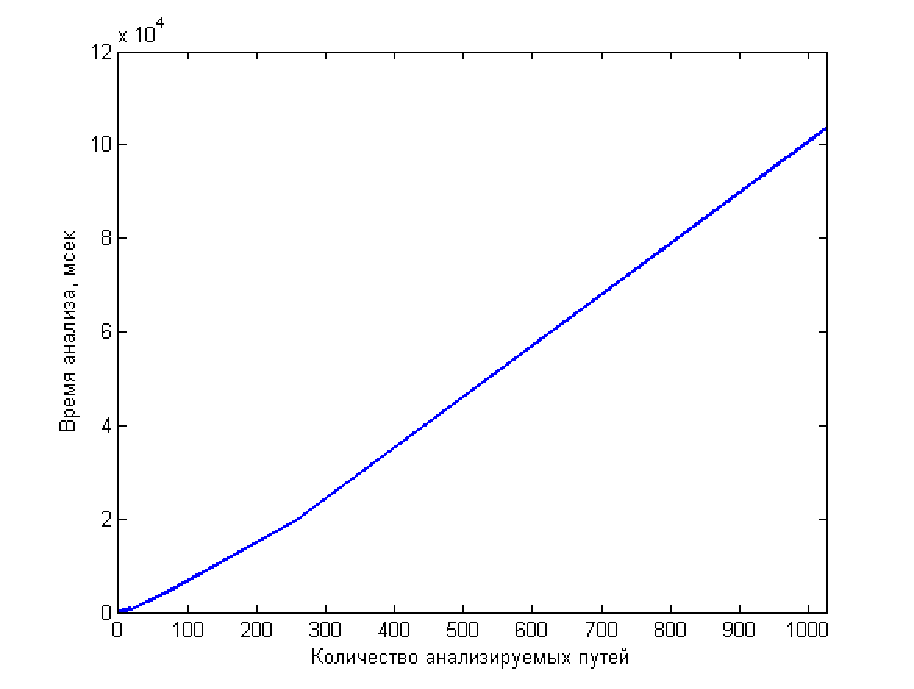
\includegraphics[width=0.9\textwidth]{inc/png/graphic3}
  \caption{Зависимость времени анализа от количества анализируемых путей}
  \label{fig:graphic3}
\end{figure}

\begin{figure}
  \centering
  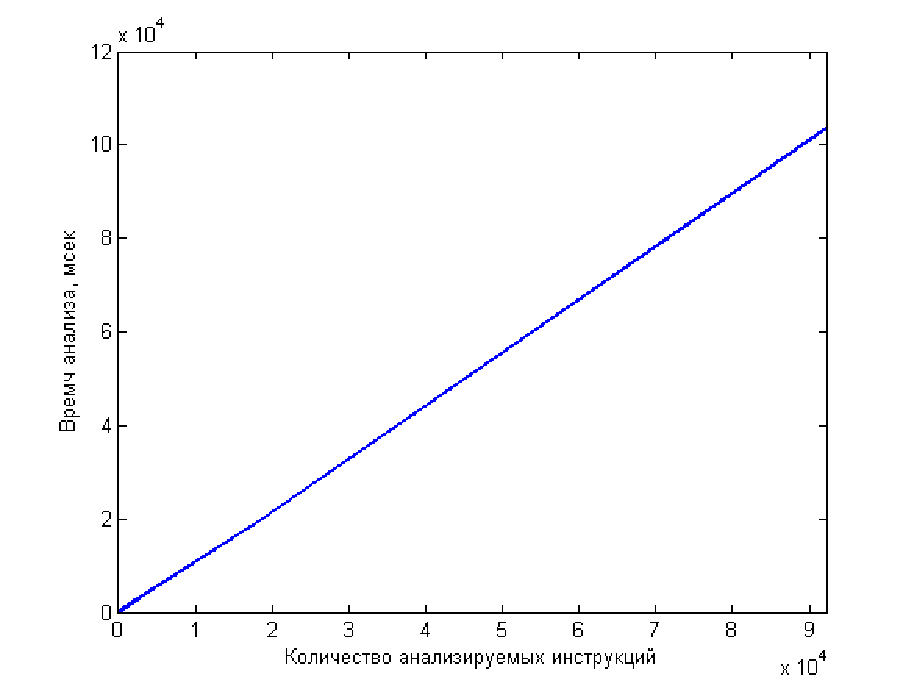
\includegraphics[width=0.9\textwidth]{inc/png/graphic4}
  \caption{Зависимость времени анализа от количества анализируемых инструкций}
  \label{fig:graphic4}
\end{figure}

\begin{figure}
  \centering
  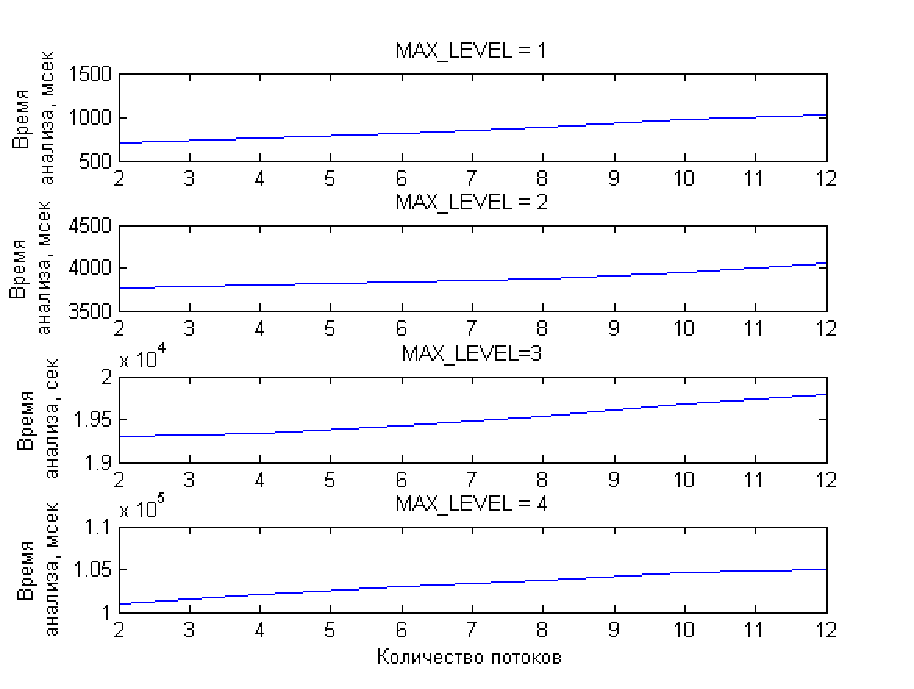
\includegraphics[width=0.9\textwidth]{inc/png/graphic5}
  \caption{Зависимость времени анализа от количества потоков}
  \label{fig:graphic5}
\end{figure}


\section{Исследование точности}

Для исследования точности получаемых результатов использовался тестовый набор программ. Рассмотрим далее результаты полученные на каждом тестовом примере, определим количество правильно обнаруженных ситуаций гонок, количества ошибок первого и второго рода.

\subsection{Программа 1}

Текст программы представлен в листинге~\ref{lst:test1}. В представленной программе в функции \textbf{main} создается 3 потока, в каждом из которых выполняется вызов функции \textbf{munge} с различными параметрами. В тексте программы отсутствуют циклы и ветвления. Анализатор выявил следующие места возникновения гонок:
\begin{verbatim}
WARNING: Race condition when accessing the variable y (global) on line 34
WARNING: Race condition when accessing the variable x (global) on line 34
WARNING: Race condition when accessing the variable z (global) on line 34
WARNING: Race condition when accessing the variable y (global) on line 8
WARNING: Race condition when accessing the variable x (global) on line 8
WARNING: Race condition when accessing the variable z (global) on line 8
\end{verbatim}
Среди найденных анализатором возможных мест возникновения гонок таковыми являются только два:
\begin{verbatim}
WARNING: Race condition when accessing the variable y (global) on line 8
WARNING: Race condition when accessing the variable z (global) on line 8
\end{verbatim}
Остальные обнаруженные места являются ошибочными и относятся к ошибками второго рода. Их появление связано с тем, что при разработке метода было сделано предположение о параллельном выполнении всех потоков программы, поэтому, хотя инициализация разделяемых переменных $x$, $y$ и $z$ выполняется в функции \textbf{main} до создания остальных потоков, анализатор берет во внимание место их инициализации и отмечает его, как потенциальное место возникновения гонок, т.к. при доступе ним не были захвачены никакие блокировки.

\lstinputlisting[language=C,caption=Программа 1(\Code{test1.c}),label=lst:test1]{inc/src/test1.c}

\subsection{Программа 2}

Текст программы представлен в листинге~\ref{lst:test2}. В представленной программе в функции \textbf{main} выпоняется создание двух потоков, в каждом из которых производится модификация глобальной переменной $x$. В одном из потоков захват блокировки, доступ к глобальной переменной и освобождение блокировки происходит в случае, когда выполняется определенное условие. Анализатор не выявил мест возникновения гонок, т.к. доступ к переменной $x$ является защищенным во всех потоках.

\lstinputlisting[language=C,caption=Программа 2(\Code{test2.c}),label=lst:test2]{inc/src/test2.c}

\subsection{Программа 3}

Текст программы представлен в листинге~\ref{lst:test3}. В программе создается 2 потока, в каждом из которых происходит чтение и печать на экран значения глобальной $x$. Анализатор не выявил мест возникновения гонок, т.к. к разделяемой переменной $x$ производился доступ только для чтения.

\lstinputlisting[language=C,caption=Программа 3(\Code{test3.c}),label=lst:test3]{inc/src/test3.c}

\section{Программа 4}

Текст программы представлен в листинге~\ref{lst:readers-writers}. Программа является решением задачи <<читатели-писатели>>. Анализатор выявил следующие места возникновения гонок:
\begin{verbatim}
WARNING: Race condition when accessing the variable buffer (global) on line 37
WARNING: Race condition when accessing the variable buffer (global) on line 19
\end{verbatim}
Оба найденные места возникновения гонок при доступе к разделяемой переменной $buffer$ являются ошибочными и относятся к ошибкам второго рода. Их появление вызвано тем, что блокировка $reader\_mutex$ захватывается не на всех анализируемых путях при доступе к переменной $buffer$. Это связано с тем, что все пути анализируются независимо друг от друга.

\section{Выводы}

Проведены эксперименты с разработанным ПО. По итогам проведенных экс­периментов определено, что разработанный метод допускает обнаружение ложных ситуаций гонок в ситуациях, когда не производится явного входа в крити­ческую секцию путем захвата какого-либо объекта блокировки, например, при условной блокировке. Кроме того в силу предположении о параллельном выполнении всех потоков, метод также допускает обнаружение ложных ситуаций гонок в ситуациях, когда выполняется только один поток, например, при инициализации переменных в главном потоке до порождения остальных потоков. На основе экспериментальных данных получена зависимость времени анализа от количества анализируемых путей, количества анализируемых инструкций и количества анализируемых потоков для задачи <<читатели-писатели>>.
